
\section{The LRC Circuit}

Name \rule{2.0in}{0.1pt}\hfill{}Section \rule{1.0in}{0.1pt}\hfill{}Date
\rule{1.0in}{0.1pt}

\textbf{Objective}

To investigate the relationships among the voltages in a series LRC
circuit.

\textbf{Apparatus} 

\begin{itemize}
\item DataStudio 750 Interface
\item AC/DC Electronics Laboratory
\item Resistor (10$\Omega$)
\item Inductor and iron core 
\item Capacitor (100$\mu F$)
\item Voltage sensors (3)
\item LRC Circuit activity
\item Wires to complete the circuit
\end{itemize}
\textbf{Introduction} 

In this exercise you will investigate a series LRC circuit through
measurements of the voltage across the generator, the resistor, the
capacitor, and the inductor in the circuit. The computer will be used
as a storage oscilloscope to make these measurements and to illustrate
the phase relationships among the voltages across the circuit elements.

Consider the series LRC circuit shown in the figure below with a generator
of voltage amplitude V, a resistor $R$, a capacitor $C$, and an inductor
having inductance $L$ and resistance $r$. Note that the capacitor is assumed
to have no resistance. Also shown in the figure is the phasor diagram
for the voltages V, V\( _{R} \), V\( _{C} \), V\( _{L} \), and
V\( _{r} \). From the phasor diagram, we can write the following
expressions:

\[
V=\sqrt{(V_{L}-V_{C})^{2}+(V_{R}+V_{r})^{2}}\]


\[
\tan \phi =\frac{V_{L}-V_{C}}{V_{R}+V_{r}}\]


\vspace{0.3cm}
{\centering \resizebox*{0.75\textwidth}{!}{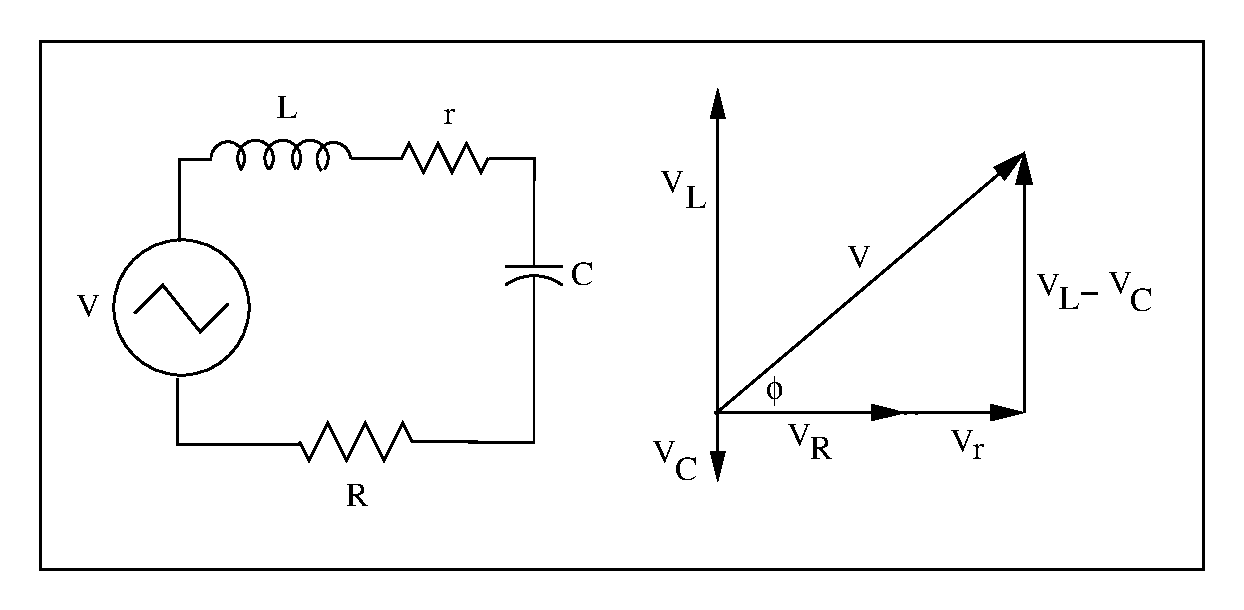
\includegraphics{lrc_circuit_fig_1.eps}} \par}
\vspace{0.3cm}

It is not possible to measure either V\( _{L} \) or V\( _{r} \)
directly. The only voltage associated with the inductor that can be
measured experimentally is the voltage across the inductor V\( _{ind} \)
which is the vector sum of V\( _{L} \) and V\( _{r} \).

\[
V_{ind}^{2}=V_{L}^{2}+V_{r}^{2}\]


The voltages V\( _{L} \) and V\( _{r} \) can be expressed in terms
of the current $I$ as

{\centering \( V_{L}=I\omega L \) \par}

{\centering \( V_{r}=Ir \)\par}

If the above expressions for \( V_{ind}^{2} \), V\( _{L} \), and
V\( _{r} \) are combined, and the current $I$ is eliminated it can
be shown that

\[
V_{L}=V_{ind}\frac{\omega L}{\sqrt{(\omega L)^{2}+r^{2}}}\]


\[
V_{r}=V_{ind}\frac{r}{\sqrt{(\omega L)^{2}+r^{2}}}\]


Assuming that \( \omega  \), $L$, and $r$ are known, V\( _{L} \) and
V\( _{r} \) can be determined from the two expressions above if V\( _{ind} \)
is measured. These values of V\( _{L} \) and V\( _{r} \) combined
with measured values of V\( _{C} \) and V\( _{R} \) can be used
in the expression for V to verify the relationship between these quantities
and the measured generator voltage V.

\textbf{Activity 1: Voltage in the LRC Circuit }

In this laboratory you will be using a voltage source that varies
sinusoidally in time.
What will the voltage from this source look like as a function
of time?
In the space below sketch your answer.
What is the phase relationship between the source voltage and the
voltage drop across an inductor?
Sketch that relationship on the same graph below.
Label your curve $V_{ind}$.
What is the phase relationship between the source voltage and the voltage
drop across a capacitor?
Again, sketch your answer on the graph below and label it $V_C$.
Finally, what is the phase relationship between the voltage drop
across a resistor in the LRC circuit and the source voltage?
Sketch it below and label it $V_R$.

\vspace{0.3cm}
{\centering \resizebox*{0.75\textwidth}{!}{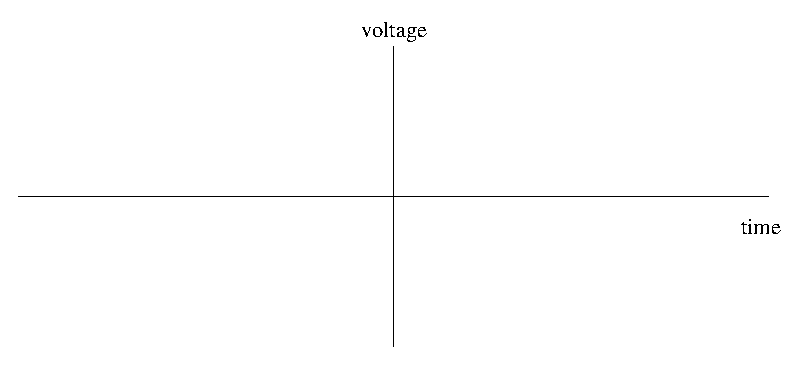
\includegraphics{lrc_circuit_fig_2.eps}} \par}
\vspace{0.3cm}

\newpage

\textbf{Activity 2: Analysis of the LRC Circuit }

(a) Construct a data table with 2 columns and 10 rows. In the first
column, label the rows C (\( \mu  \)F), V (V), V\( _{R} \) (V),
V\( _{ind} \) (V), V\( _{C} \) (V), V\( _{L} \) (V), V\( _{r} \)
(V), \( \phi  \) (deg), \( \sqrt{(V_{L}-V_{C})^{2}+(V_{R}+V_{r})^{2}} \)
(V), and \% Diff.
\vspace{5in}

(b) Open the \emph{LRC Circuit} activity
in the 132 Workshop folder in the Programs menu. 
Go to the `Signal Generator' window and set the frequency to 30 Hz, the amplitude 
to 3.0 V, and the wave form to `Sine Wave'.
If you can't find the `Signal Generator' window, click the `setup' button at
the top of the DataStudio menu.
You will see an image of the Pasco 750 interface with several
connections marked.
Single click on the one called `Output'.
The `Signal Generator' window should pop up. 
Set the values on it and return to the original voltage graph window.

(c) Set up the circuit on the AC/DC Electronics Laboratory so that it corresponds to the one
shown in the first figure above. The iron core (a long metal cylinder)
should be inserted in the inductor.
The inductor is the large open, cylinder in the upper-right-hand part of
of the AC/DC Electronics Laboratory.
The computer and the circuit are set up to measure the voltage
across each of the circuit elements. The resistor in the circuit 
has a value $R=10\Omega$. Check this value with the DMM and record it
as $R$ on your data sheet. In the last lab you determined the inductance
$L$ and resistance $r$ of your inductor. Record these values in the space
below. Use the value for $r$ measured with the DMM in the previous experiment.
Record the value of the capacitor (100 \( \mu  \)F) in your data table.
\vspace{15mm}

(d) Take data! The computer will display four sinusoidal
voltage signals. 
The color scheme to identify each voltage measurement
is shown on the right of the voltage graph window. Determine which trace
corresponds to V (the source signal), V\( _{R} \) (the resistor voltage),
V\( _{C} \) (the capacitor voltage), and V\( _{ind} \) (the inductor voltage).
Examine
the phase relationships among the signals. Do these relationships
agree with the phasor diagram in the above figure? Explain.
Do they agree with the predictions you made in Activity 1?
Explain any differences.
\vspace{20mm}

(e) Measure the amplitude of each of the signals and record these
quantities in your data table. This can be done using the SmartTool graph
accessory (see Appendix B), or read directly from the graph.

(f) Calculate the remaining quantities necessary to complete the data
table. The \% Diff should be determined between the measured value
for the generator voltage V and \( \sqrt{(V_{L}-V_{C})^{2}+(V_{R}+V_{r})^{2}} \).
Show the calculations in the space below. Do your
results confirm the phasor diagram shown in the figure above as a
correct model for the addition of voltages in an LRC circuit? Explain.
\vspace{4in}

(g) Construct to scale a phasor diagram like the one shown in the
figure above, based on your data. Choose some scale (for example
1.00 V/cm) so that the diagram is as large as possible, but still fitting 
in the space below. Are the phase relationships consistent
with what was observed on the computer screen? Is the phase angle
\( \phi  \) consistent with the calculated value?
\vspace{3.5in}

\textbf{Activity 3: Resonance in the LRC Circuit }

(a) Construct a data table with the column headings f (Hz),
V\( _{R} \) (V), and I\(_R \) (A) in the space below.
\vspace{3in}

(b) Set the frequency of the generator to 30 Hz and record this
frequency in your data table. Take data for a few seconds and stop. You may
have to adjust the horizontal scale to see at least two complete
cycles of the signals. Use the button on the horizontal axis.
Measure V\( _{R} \)  and record it in your data table. (Note: If the peaks 
of the curves appear
to be cut off, reduce the input amplitude and repeat the measurements.)

(c) Repeat step (b) for frequencies of 50, 70, 80, 90,
100, 110, 130, 150, 170, 200, 250, 300, and 350 Hz. The \textbf{}horizontal scale \textbf{}should
be adjusted so that at least two cycles of the signals can be viewed.
Examine the change in the phase relationship between the signals as
the frequency is changed. 

(d) Record V\( _{R} \)  for each
frequency in the second data table. What is resonating in the
circuit? Calculate I\(_R\) for each entry in your table.
Construct a graph of I\( _{R} \)
(y axis) versus frequency and insert it into your notebook. Calculate
the resonant frequency that you would expect from the values of $L$
and $C$ in the circuit. Does the calculated value for the resonant frequency
agree with the graph? Explain.
\vspace{40mm}

(e) Set the frequency of the generator to the resonant
frequency and use the LRC Circuit activity to display the
four voltage signals. Describe and explain the phase relationships
among the signals at resonance. Compare them with the predictions
you made earlier. \vspace{20mm}

